\documentclass[slidestop, compress, mathserif]{beamer}
\usepackage[style=authoryear-comp, sorting=nyt, maxcitenames=2, backend=biber]{biblatex}
\renewbibmacro{in:}{}
\renewcommand\bibfont{\small}
\addbibresource{ref_01.bib}
\addbibresource{ref_02.bib}
\addbibresource{ref_03.bib}
\addbibresource{trappe.bib}

\usepackage{amsmath, amssymb, mathrsfs}
\usepackage{color, graphicx}

\usepackage{setspace, listings}
\usepackage{sidecap}

\usetheme{Madrid}
\usecolortheme{default}
\linespread{1.2}



\sidecaptionvpos{figure}{c}
\usepackage[textfont=small]{caption}
\setbeamertemplate{caption}[numbered]
\captionsetup{font=scriptsize, labelfont=scriptsize, labelformat=simple}

\setbeamertemplate{footline}
{
  \leavevmode%
  \hbox{%
  \begin{beamercolorbox}[wd=1.0\paperwidth,ht=2.25ex,dp=1ex]{author in head/foot}\usebeamerfont{author in head/foot}
    \hspace*{3ex}
    \inserttitle
    \hfill
    \insertshortauthor
    \hspace*{3ex}
  \end{beamercolorbox}%
}%
  \vskip0pt%
}


% \institute{DICMaPI, University of Naples Federico II}
% \author{Gun Woo Park, Antonio Brasiello, and Giovanni Ianniruberto}
% \date{SUPOLEN PROJECT MEETING\\ 27 MAR 2015}


% it's for headline
% \setbeamertemplate{headline}{%
%   % \leavemode%
%   \hbox{%
%     % \begin{beamercolorbox}[wd=\paperwidth,ht=2.5ex,dp=1.125ex]{palette quaternary}%
%     \begin{beamercolorbox}[wd=\paperwidth,ht=2.5ex,dp=1.125ex]{section in head/foot}%
%       \insertsectionnavigationhorizontal{\paperwidth}{}{\hskip0pt plus1filll}
%     \end{beamercolorbox}%
%     }
% }

\begin{document}
\title{Data Processing for ICR Abastract}
\author{Gun Woo Park}

\begin{frame}[plain]
\maketitle
\end{frame}

\begin{frame}
  \frametitle<presentation>{Chain Number Density, $\nu$}
  \begin{block}{Reported data in Suzuki et al. (2012)}
    \begin{align}
      \nu &\approx 3.7 \times 10^{21}/m^3 \quad\textrm{number density for active chains}\\
      \nu_0 &= 1.8 \times 10^{23}/m^3\quad\textrm{number density for all chains}
    \end{align}
    Note that $R_0 \in [1, 30]nm$, which implies $\nu_0R_0^3 \in [1.8\times 10^{-4}, 4.86]$.
  \end{block}
  The given condition:
  \begin{itemize}
    \item Number of chains per particles = 25
    \item Number of particles = 400, 600, 800, 1000, 1200, 1400
    \item Volume of box = $10^{3}R_0^3$
  \end{itemize}
  Measured number density: $\nu_xR_0^3 = \{10,\, 15,\, 20,\, 25,\, 30,\, 35\}$
\end{frame}

\begin{frame}
  \frametitle<presentation>{Chain Number Density, $\nu$ (cont.)}
  \begin{block}{Expectated Micelle Dimension}
  \begin{equation}
    \nu_{x} R_0^3 = F \Rightarrow R_0/nm = \left(\frac{F}{\tilde{\nu}_0}\right)^{1/3} = \left(\frac{F}{1.8}\times 10^{4}\right)^{1/3}
  \end{equation}
  \end{block}
  Underline this aspect, the test condition $\nu_xR_0^3 = \{10,\, 15,\, 20,\, 25,\, 30,\, 35\}$ means the expected dimensions are 38.2, 43.7, 48.1, 51.8, 55.0, and 57.9 in $nm$.
  % \begin{block}{Expected Aggregation Number per Micelles, Yekta et al. (1995)}
  %   Number of \textit{chain ends} per micelles are expected around 20 with slightly different HEUR structure.
  % \end{block}

  If we reduce the number of chains per micelle from 25 to 10, we have number new number density cases with the existing number of particles: $\nu_nR_0^3 = \{4,\, 6,\, 8,\, 10,\, 12,\, 14\}$, which implies the expected dimension for micelles as 28, 32, 35, 38, 40, and 42 in $nm$.

\end{frame}

\begin{frame}
  \frametitle<presentation>{Stress Autocorrelation Function (semilog)}
  \begin{figure}
    \centering
    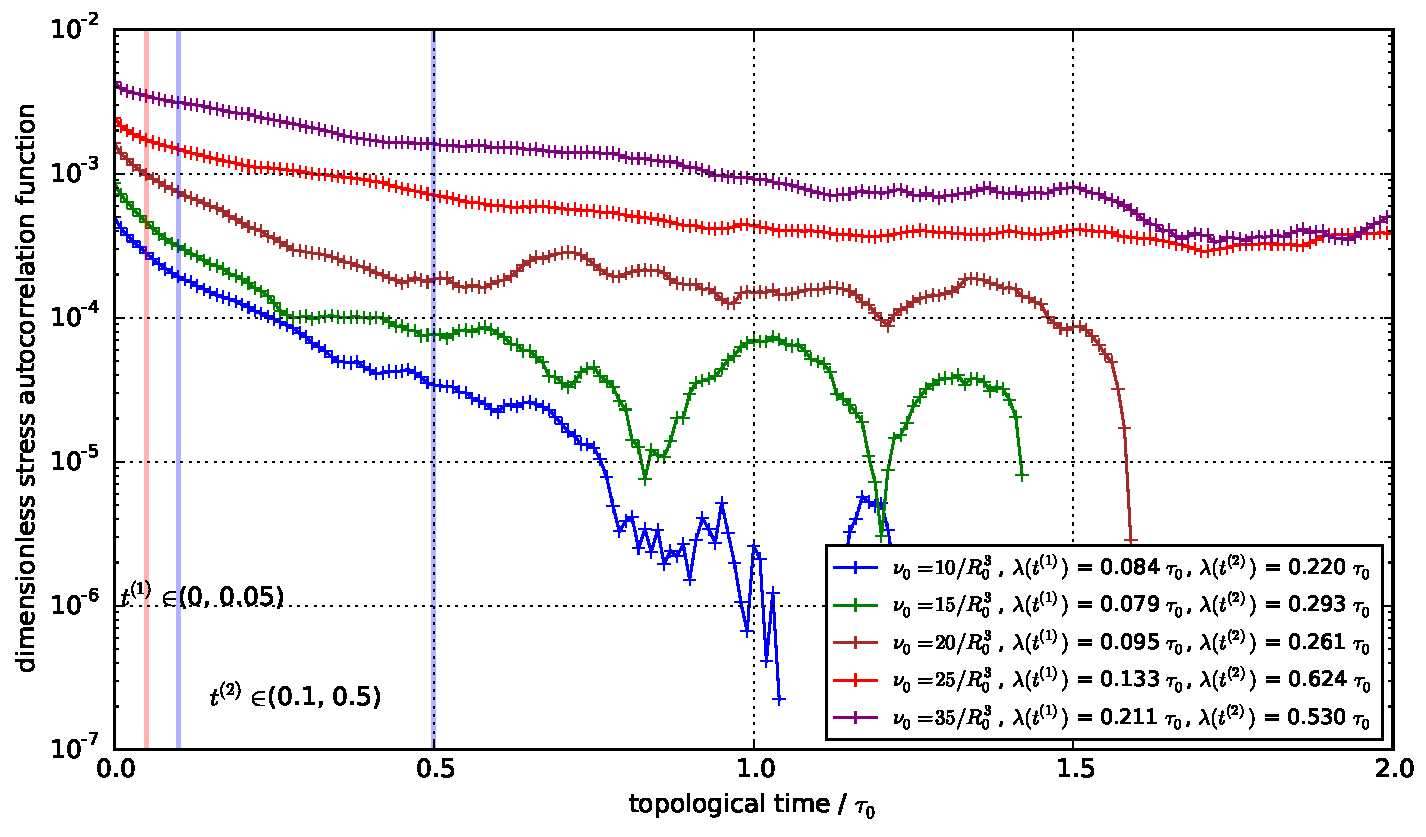
\includegraphics[width=\textwidth]{figures/stress_autocorrelation_ICR_abstract.pdf}
  \end{figure}
\end{frame}

\begin{frame}
  \frametitle<presentation>{Stress Autocorrelation Function (semilog)}
  \begin{figure}
    \centering
    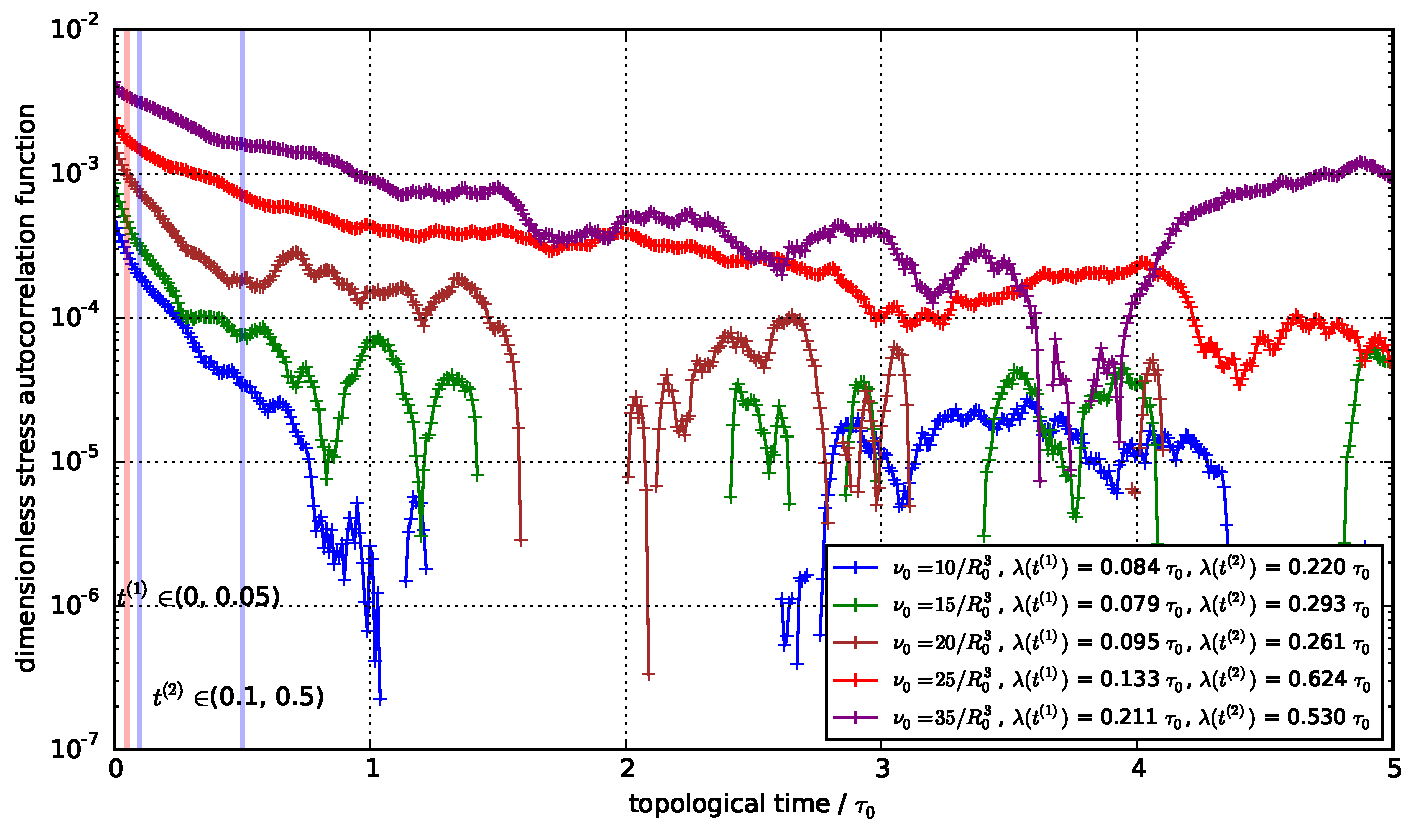
\includegraphics[width=\textwidth]{figures/temporal_report_pre_semilogy.pdf}
  \end{figure}
\end{frame}

\begin{frame}
  \frametitle<presentation>{Temporal Results for RT=10k, NP=400}
  \begin{figure}
    \centering
    \includegraphics[width=0.45\textwidth]{../../../tmp/NP400_RT10k_ACF_linear.pdf}
    \includegraphics[width=0.45\textwidth]{../../../tmp/NP400_RT10k_ACF_semilogy.pdf}
  \end{figure}
\end{frame}


% \begin{frame}
%   \frametitle<presentation>{Stress Autocorrelation Function (semilog, longer)}
%   \begin{figure}
%     \centering
%     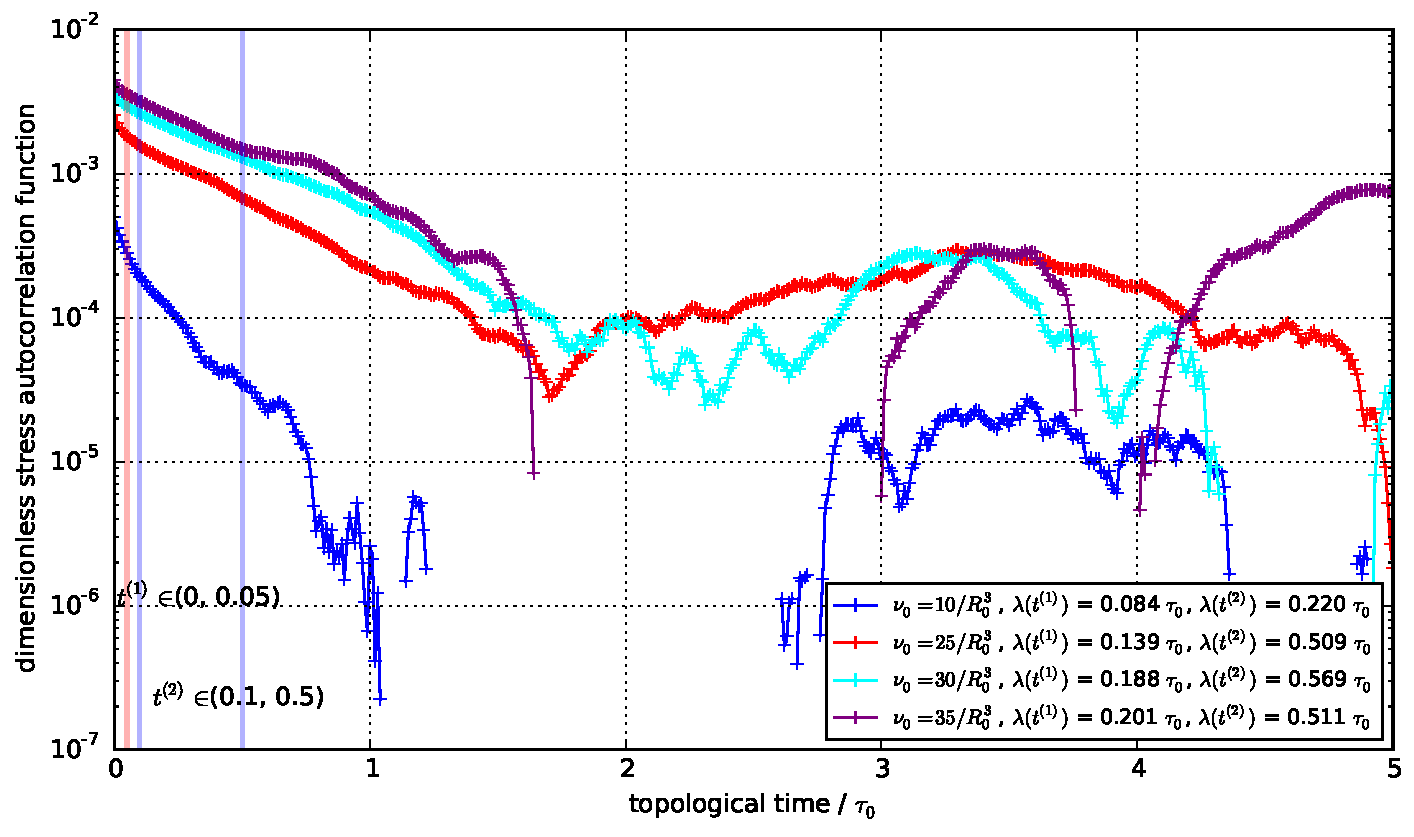
\includegraphics[width=\textwidth]{../../equilibrium_analysis_dt0_01/temporal_report_semilogy.pdf}
%   \end{figure}
% \end{frame}

% \begin{frame}
%   \frametitle<presentation>{Stress Autocorrelation Function (double log, longer)}
%   \begin{figure}
%     \centering
%     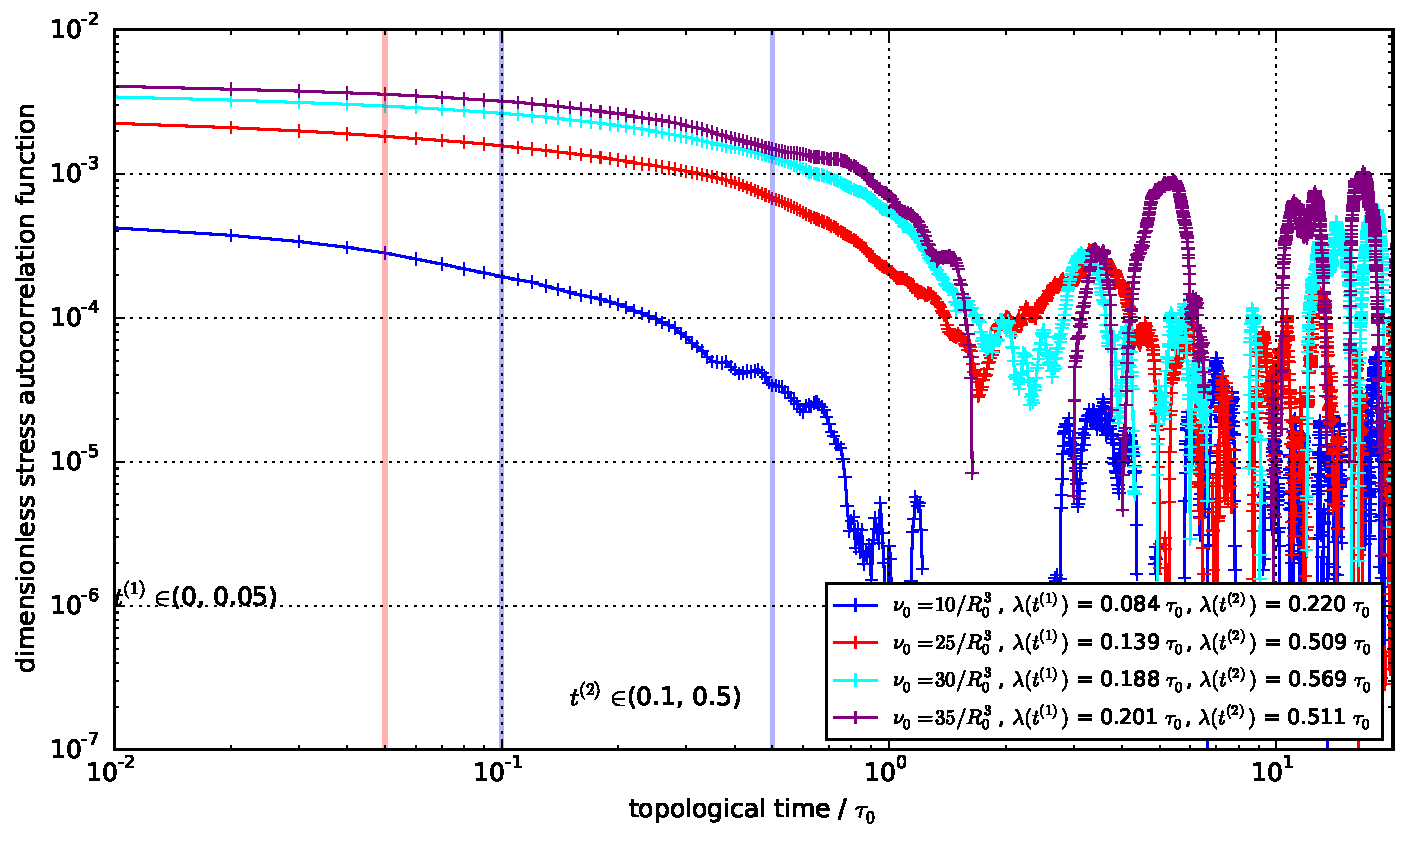
\includegraphics[width=\textwidth]{../../equilibrium_analysis_dt0_01/temporal_report_loglog.pdf}
%   \end{figure}
% \end{frame}


% \begin{frame}
%   \frametitle<presentation>{ACF, legend change}
%   \begin{figure}
%     \centering
%     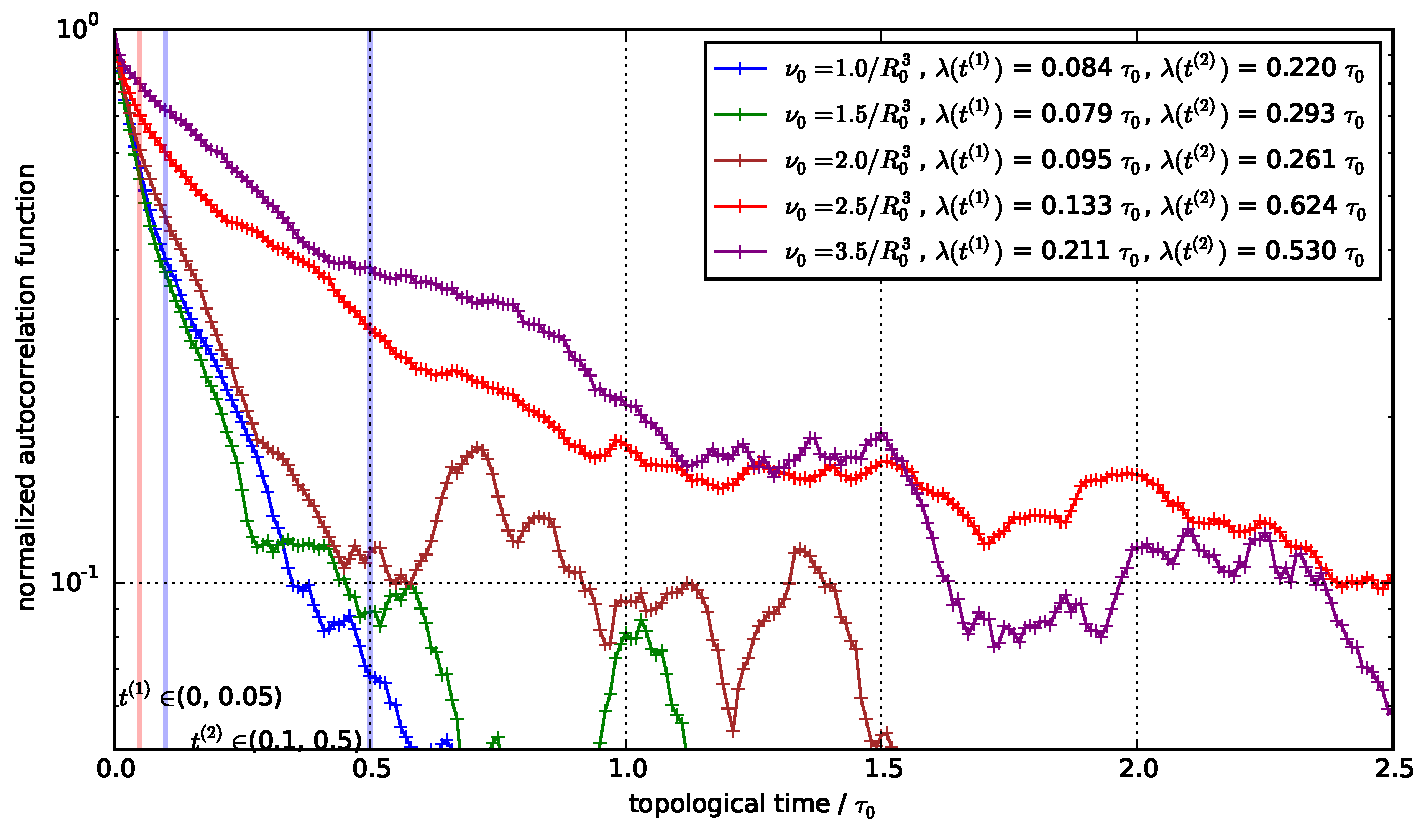
\includegraphics[width=\textwidth]{../../equilibrium_analysis_dt0_01/check_ACF_semilogy_ICR_abstract.pdf}
%   \end{figure}
% \end{frame}

% \begin{frame}
%   \frametitle<presentation>{Number of Distingushable Association, Functionality}
%   \begin{figure}
%     \centering
%     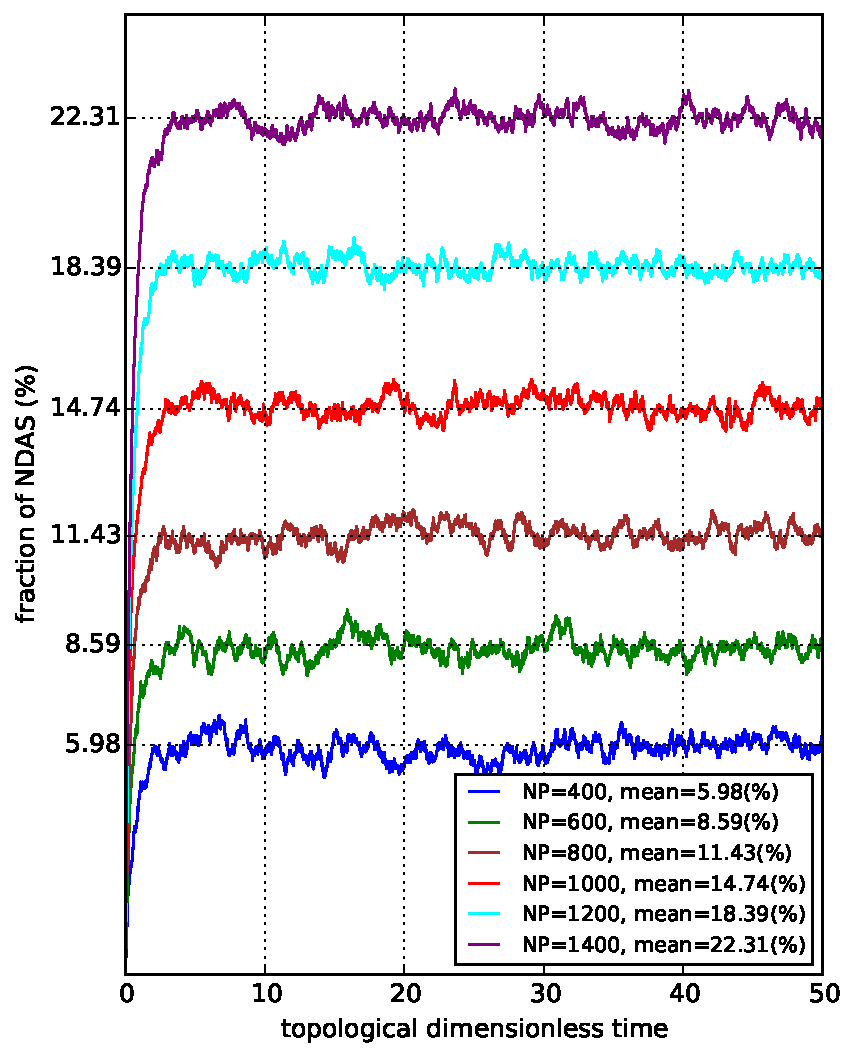
\includegraphics[width=0.45\textwidth]{../../equilibrium_analysis_dt0_01/check_fNDAS.pdf}
%     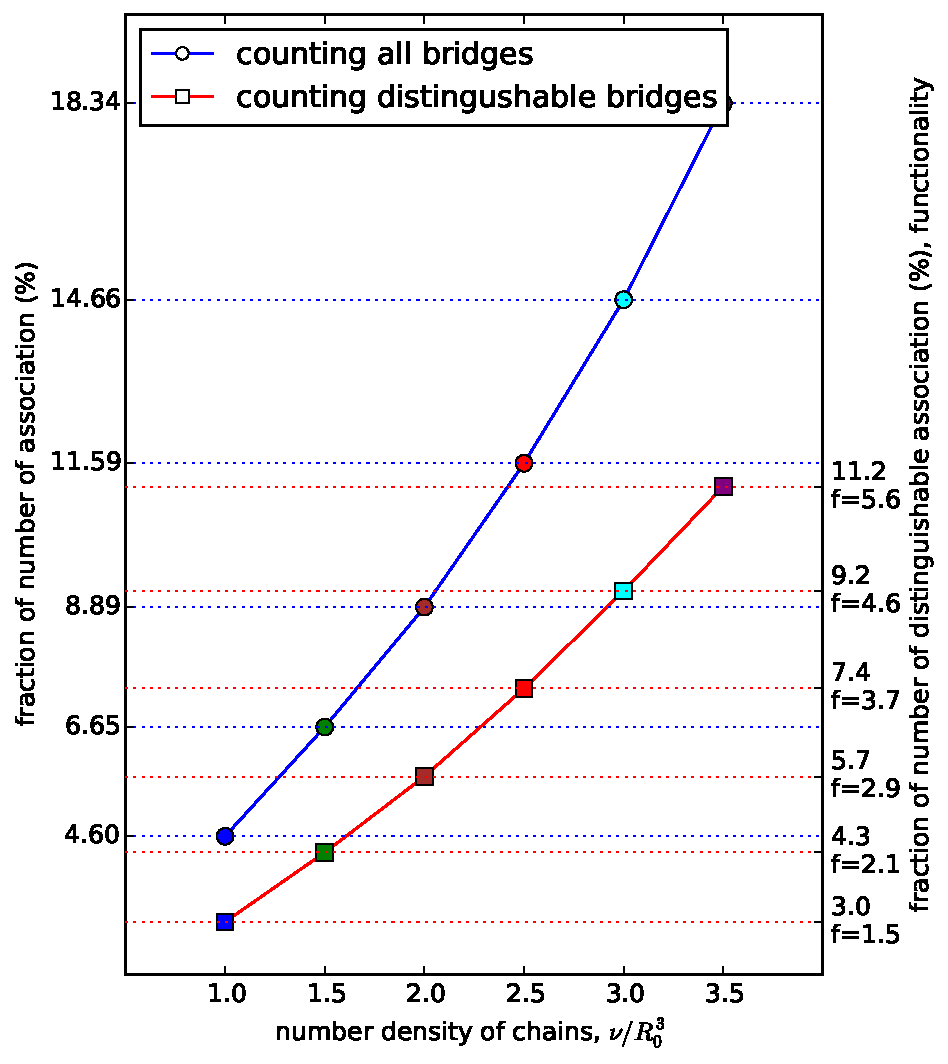
\includegraphics[width=0.45\textwidth]{../../equilibrium_analysis_dt0_01/check_fNAS_fNDAS.pdf}
%   \end{figure}
% \end{frame}

% \begin{frame}
%   \frametitle<presentation>{Relaxation Time Spectrum}
%   \begin{block}{Continuous relaxation time spectrum}
%     \begin{equation}
%       G(t)=\sum_i G_i \exp\left(-\frac{t}{\lambda_i}\right) \quad\Rightarrow\quad G(t) = \int_0^\infty H(\lambda)\exp\left(-\frac{t}{\lambda}\right)d\log \lambda,
%     \end{equation}
%     where $H(\lambda)$ is called relaxation time spectrum.
%   \end{block}
%   \vspace{-0.2in}
%     \begin{align}
%       G^\prime (\omega) &= \int_0^\infty H(\lambda)K^\prime (\lambda \omega) d\log\lambda\\
%       G^{\prime\prime} (\omega) &= \int_0^\infty H(\lambda)K^{\prime\prime} (\lambda \omega) d\log\lambda
%     \end{align}
%     with 
%     \begin{equation}
%       K^{\prime}(\lambda \omega) = \frac{\lambda^2\omega^2}{1+\lambda^2\omega ^2} \quad K^{\prime\prime}(\lambda \omega) = \frac{\lambda\omega}{1+\lambda^2\omega ^2}.
%     \end{equation}
    




% \end{frame}

% \begin{frame}
%   \frametitle<presentation>{Dynamic Moduli, Reproduced from Suzuki et al. (2012)}
%   \begin{figure}
%     \centering
%     \includegraphics[width=\textwidth]{/Users/parkgunwoo/Dropbox/works/RTD/dist_fixed_point/last_version/HEUR_solution/check_dynamic_moduli.pdf}
%   \end{figure}
% \end{frame}

% \begin{frame}
%   \frametitle<presentation>{Relaxation Time Spectrum, Cho and Park (2013)}
%   \begin{figure}
%     \centering
%     \includegraphics[width=\textwidth]{/Users/parkgunwoo/Dropbox/works/RTD/dist_fixed_point/last_version/HEUR_solution/check_RTD.pdf}
%   \end{figure}
% \end{frame}


% \begin{frame}[plain]
% \title{Performance Check}
% \author{Gun Woo Park}
% \maketitle
% \end{frame}



% \begin{frame}
%   \frametitle<presentation>{Test Condition, larger time step}
%   \begin{block}{Current definition for time scales}
%   \begin{align}
%     \tau_0 &= \beta_0^{-1}\quad\textrm{dissociation time}\\
%     \tau_B &= \frac{R_0^2\zeta}{k_BT}\frac{1}{C},\quad\textrm{Brownian time}.
%   \end{align}
%   As a default, the rational time scale, $R_t = \tau_0/\tau_B$, is set by 100.
%   \end{block}
%   \begin{itemize}
%   \item time step for Brownian motion: $10^{-4}\tau_0$ (=$10^{-2}\tau_B$) $\Rightarrow$ $10^{-3}\tau_0$ (=$10^{-1}\tau_B$)
%   \item time step for topology: $10^{-3}\tau_0$ $\Rightarrow$ $10^{-3}\tau_0$ and $10^{-2}\tau_0$
%   \item data output frequency: $10^{-2}\tau_0$ 
%   \end{itemize}
% \end{frame}

% \begin{frame}
%   \frametitle<presentation>{ACF, failed to match}
%   \begin{figure}
%     \centering
%     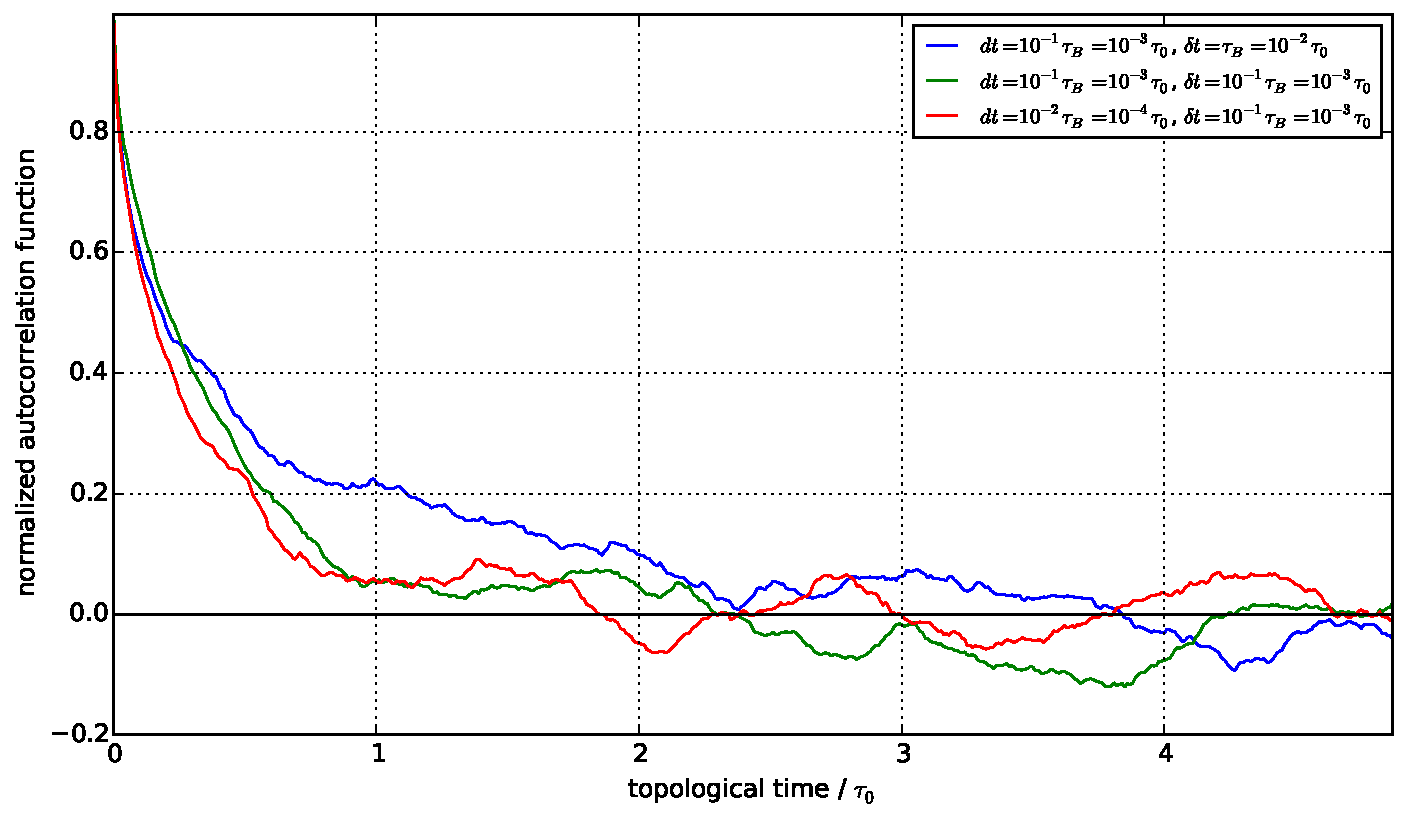
\includegraphics[width=\textwidth]{check_performance_ACF.pdf}
%   \end{figure}
% \end{frame}

% \begin{frame}
%   \frametitle<presentation>{Shear Stress}
%   \begin{figure}
%     \centering
%     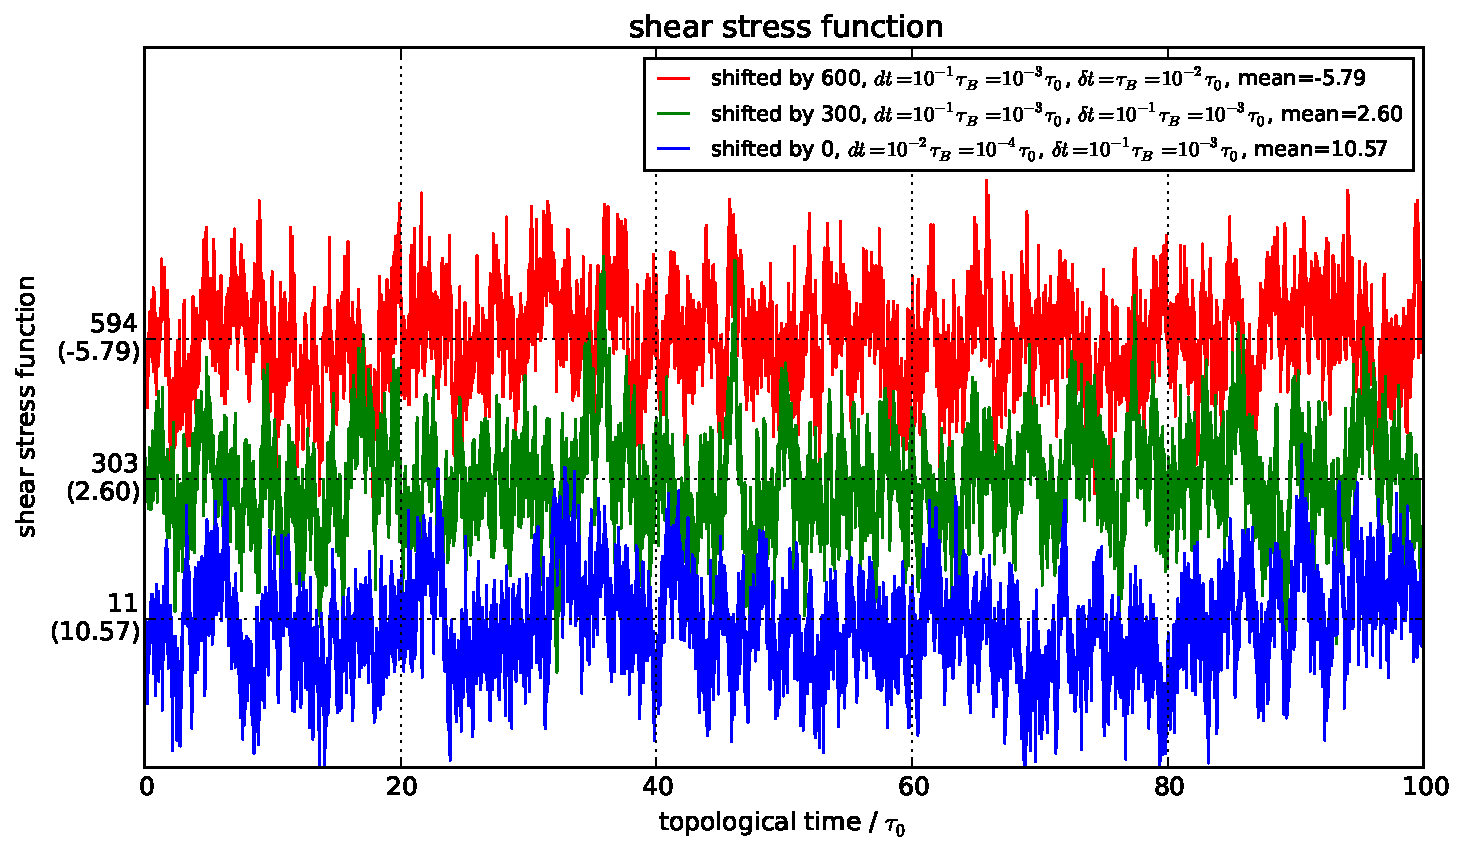
\includegraphics[width=\textwidth]{check_performance_shear_stress.pdf}
%   \end{figure}
% \end{frame}

% \begin{frame}
%   \frametitle<presentation>{ACF, failed to match}
%   \begin{figure}
%     \centering
%     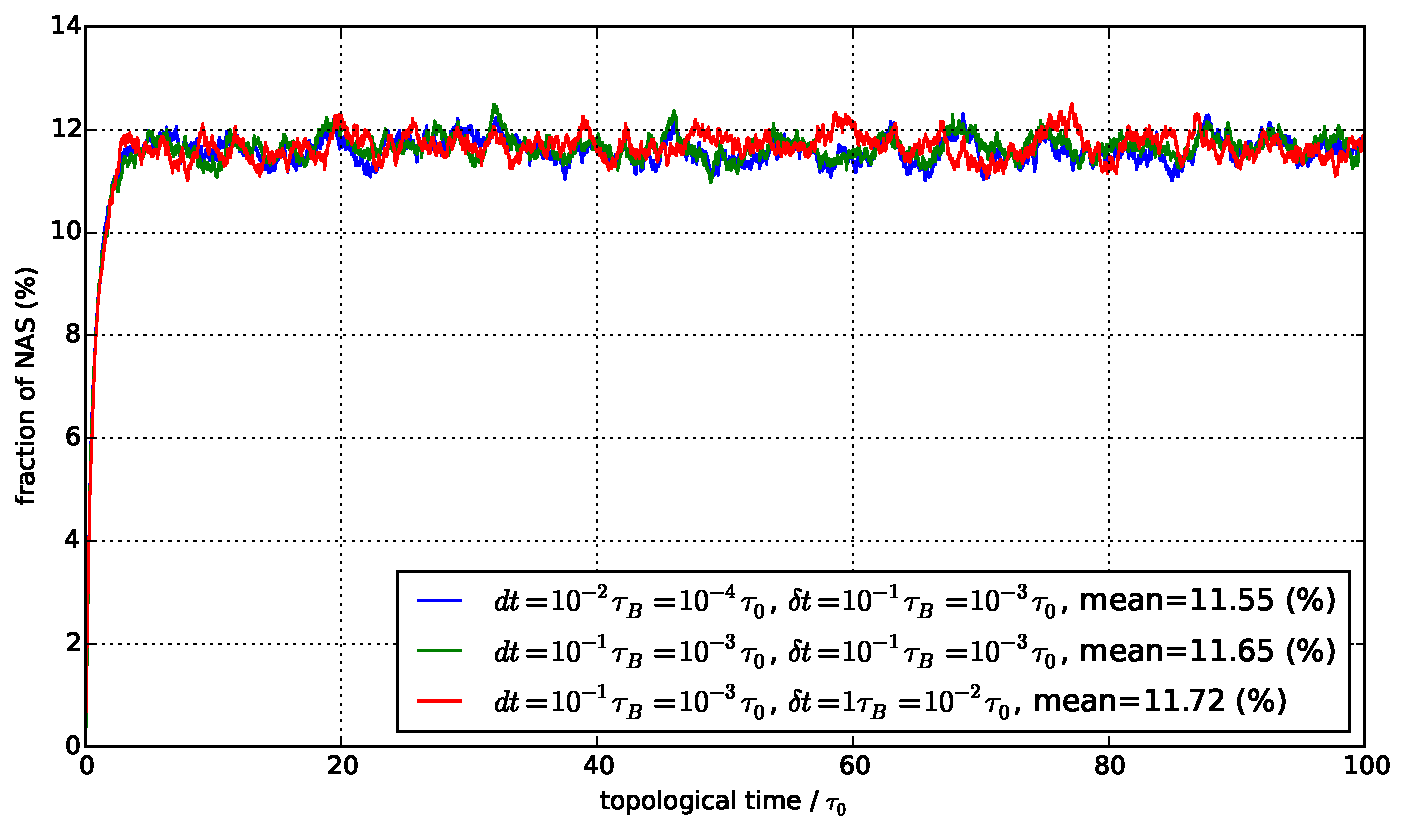
\includegraphics[width=\textwidth]{../check_performance_fNAS.pdf}
%   \end{figure}
% \end{frame}

\begin{frame}
  \frametitle<presentation>{equation}
  $$ \delta t$$
$$ \beta $$
$$ \beta_0 $$
$$ R_0 $$
$$ R_0^3 $$

  \begin{equation}
    \frac{\partial \mathbf{r}_k}{\partial t} = \frac{1}{\zeta} \left(\sum_{i\in\mathscr{C}_k} \mathbf{F}^{(el)}(\mathbf{r}_{i}, \mathbf{r}_k) + \sum_{i=1}^{N_p}\mathbf{F}^{(rep)}(\mathbf{r}_i, \mathbf{r}_k) + \mathbf{F}^{(B)}(\mathbf{r}_k)\right),
  \end{equation}
  \begin{equation}
    P^{dissoc} = \beta\delta t = \beta_0 \exp\left(\frac{F^{(el)}l_c}{k_BT}\right)\delta t,
  \end{equation}
\end{frame}


\end{document}